\documentclass[11pt]{article}
\renewcommand{\baselinestretch}{1.05}

\usepackage{amsmath,amsthm,verbatim,amssymb,amsfonts,amscd, graphicx}
\usepackage{graphics}

\usepackage{xcolor}

\usepackage[hidelinks]{hyperref}

\usepackage{parskip}

\renewcommand{\contentsname}{Table des mati\`eres}

\topmargin0.0cm
\headheight0.0cm
\headsep0.0cm
\oddsidemargin0.0cm
\textheight23.0cm
\textwidth16.5cm
\footskip1.0cm

\begin{document}

\title{\textbf{TP Caract\'erisation} }
\author{Lucien Dos Santos \\ Mohamed Hage Hassan}
\date{21 Mars, 2017}
\maketitle

\tableofcontents
\clearpage

\section{Introduction}

\section{Description G\'en\'erale}

Le but principal de ce TP est de caract\'eriser les 2 composantes principales du transistor MOS :

\begin{figure}[!htb]
\centering
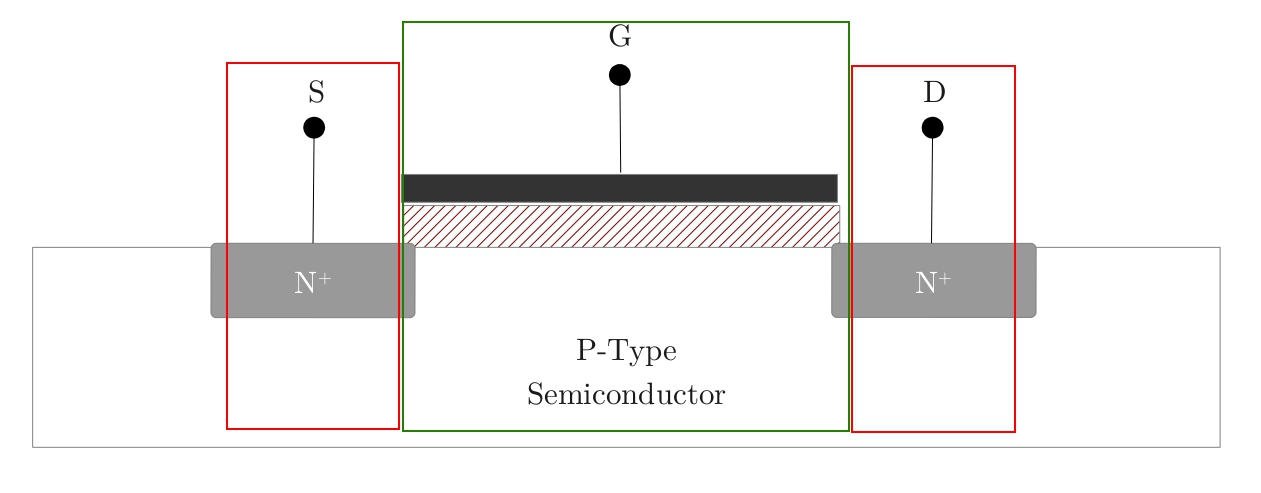
\includegraphics[scale=0.30]{mosfet_structure_implemented_side_view.jpg}
\caption{Composition du MOSFET}
\end{figure}

La capacit\'e MOS (vert) et les 2 jonctions PN (rouge) r\'esultantes des manipulations effectu\'ees en salle blanche.
On sp\'ecifie que ces 2 parties peut-\^etre utilis\'ees comme des composantes seules :

\begin{itemize}
\item \textbf{Jonction PN}

\begin{itemize}
\item[-] Capteurs thermiques (au lieu des couples thermiques).
\item[-] Capteurs optiques : photod\'eteteurs.
\item[-] Transmissions haute-fr\'equence (diode optiques).
\end{itemize}

\item \textbf{Capacit\'ees MOS}
\begin{itemize}
\item[-] Matrice de capacit\'ees MOS utilis\'ees pour la reconstruction d'une image dans les appareils photo r\'ecentes.
\end{itemize}

\end{itemize}

On note que pour la partie salle blanche, on a r\'ealiser la jonction PN :

\textbf{\'Etapes de r\'ealisation}
\begin{itemize}
\item[-] Nettoyage du wafer.
\item[-] D\'epot du $SiO_2$.
\item[-] Diffusion thermique pour le dopage du wafer (en type $n+$).
\item[-] Deposition d'une couche d'Aluminium
\item[-] Gravure d'aluminium.
\end{itemize}

\section{Caract\'erisation de la jonction PN}
On cherche \`a d\'eterminer la caract\'eristique I/V de la jonction.
L'allure g\'en\'erale du courant d'une diode en fonction de la tension est r\'epr\'esent\'ee par le sch\'ema suivant :

\begin{figure}[!htb]
\centering
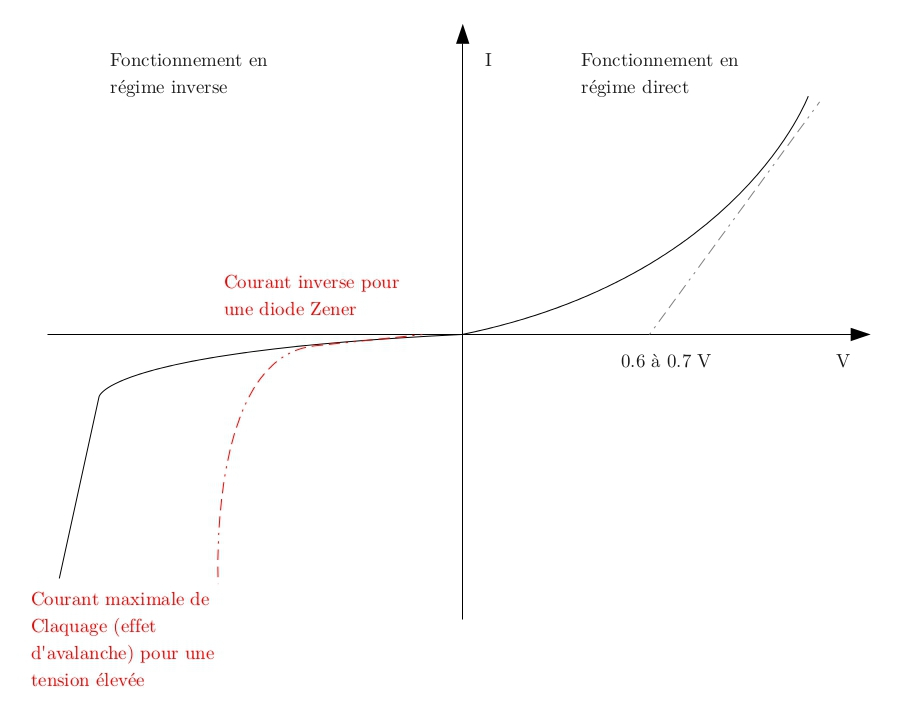
\includegraphics[scale=0.54]{carac_I_V.jpg}
\caption{R\'egime du foncitonnement de la jonction PN}
\end{figure}

On souhaite donc chercher les param\`etres : 
\begin{itemize}
\item[-] $I_S$ courant de saturation
\item[-] $V_{th}$ Tension de seuil (Thershold volatage)
\item[-] $V_a$  Tension d'avalanche
\item[-] $n$ facteur d'id\'ealit\'e
\end{itemize}
\clearpage

\subsection{M\'ethodes de d\'etermination des param\`etres}

\textbf{Courant de saturation $I_S$ et du facteur n}

Sachant que le mod\`ele math\'ematique de la diode s'exprime par :
\[
	I = I_S (e^{\frac{q V}{n K_B T}} - 1 )
\]

On constate que c'est difficile de d\'eterminer la valeur de $I_{S}$ directement, sachant qu'entre 0 et 0.6V, en zone directe de fonctionnnement, on a un ph\'enom\`ene de recombinaison des porteurs (charge d'espace). Ce phenom\`ene pr\'eexiste toujours en r\'egime inverse.

Pour se faire, on prend le mod\`ele simplifi\'e de $I$ \textbf{pour la zone directe}:

\[
	I = I_S (e^{\frac{q V}{n K_B T}})
\]
\[
\implies	ln(I) = ln(I_S) +  \frac{q V}{n K_B T}
\]

On retrouve que c'est possible de d\'eterminer ces 2 facteurs :

\begin{figure}[!htb]
\centering
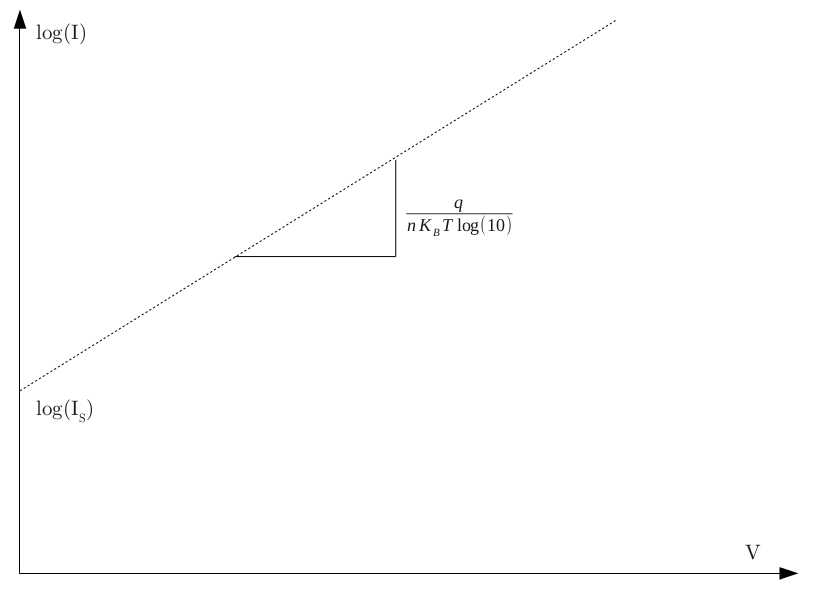
\includegraphics[scale=0.54]{log_echelle.jpg}
\caption{Passage en \'echelle logarithmique}
\end{figure}

Pour la d\'etermination de $n$, on sait que pour $n=1$, on a un $\Delta V$ de $60 \phantom{2} mV$ pour une d\'ecade. 

\textbf{D\'etermination de $V_a$ et $V_{th}$} 

$V_{th}$ constitue l'intersection de l'asymptote \`a l'exponentielle de la courbe $I_{S}$ avec l'axe $ox$, et $V_{a}$ la tension pour laquelle on a une tr\`es forte d\'erive en intensit\'e.

\subsection{Partie pratique}
Pour la caract\'erisation des diodes, on utilise le Hwelett Packard 4155A Semiconductor Parameter Analyser. On vient manipuler des pointes en carbure de tungest\`ene pour la mesure des param\`etres d'une jonction PN :

\begin{figure}[!htb]
\centering
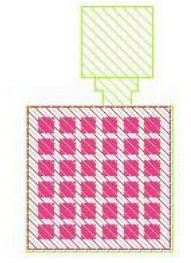
\includegraphics[scale=0.54]{diode_junction.jpg}
\caption{Diode de grande surface et petit p\'erim\`etre, surface $200 \times 200 \mu m^{2}$}
\end{figure}

La plaque principale de l'outil de mesure est polaris\'ee en inverse : on affiche les valeurs de I en fonction de V (courbe initialement \`a l'inverse), et on retrouve $V_{th} = 0.678 \phantom{2} V$ 


\section{Conclusion}




\end{document}